\documentclass{article}
\usepackage[hybrid]{markdown}
\usepackage{lineno}
\linespread{2} 
\linenumbers
\usepackage{natbib}
\usepackage{amsmath}
\usepackage{algorithm}
\usepackage{algpseudocode}
\bibliographystyle{abbrvnat}
\setcitestyle{
    authoryear,
    open={(},
    close={)}
}
\usepackage{hyperref}
\hypersetup{
    urlcolor=blue,
    colorlinks=true,
    linkcolor=black
}
\usepackage{geometry}

 \geometry{
     a4paper,
     left=25mm,
     right=25mm,
 }
 \title{Clockor2:  Inferring global and local strict molecular clocks using root-to-tip regression}

\begin{document}
\maketitle
\begin{centering}
Leo A. Featherstone$^{\ast,1}$, Sebastian Duchene$^1$, Wytamma Wirth$^{1}$\\
$^{1}$ Peter Doherty Institute for Infection and Immunity, University of Melbourne, Australia.\\
*email: leo.featherstone@unimelb.edu.au
\end{centering}

\section*{Abstract}


\section*{Introduction}
Phylodynamics achieves its greatest value when generating insight about infectious disease dynamics outside the purview of epidemiology. This frequently occurs at population interfaces, such as transmission across host sub-populations,  geographical boundaries or host species. In each case, the essential component to phylodynamic modelling is always the assumption of a molecular clock relating epidemiological and evolution.

The simplest molecular clock models are strict clocks, which assume a constant rate of substitution per unit time. We further divide these into global and local strict clocks. Global strict clocks assert one fixed molecular evolutionary rate for all samples in a tree, while local strict clocks allow for different fixed rates to apply to different portions of a tree. Clockor2 allows for fast inference of global and local strict molecular clocks from an input tree of genome sequences annotated with sampling times using root-to-tip regression (RTT). Several other tools allow for the inference of strict molecular clocks via RTT, but none readily offer the ability to fit local clocks models \citep{rambaut_exploring_2016, hadfield_nextstrain_2018,sagulenko_treetime_2018,volz_scalable_2017}. 

Phylodynamic datasets are and will continue to grow in size and scope \cite{featherstone2022epidemiological}. For example, larger than ever datasets have been used to understand the spread of SARS-CoV-2 at national and international scales, as well as study the emergence of variants of concern (VOC), and transmission to other species \citep{du_plessis_establishment_2021,hill_origins_2022,nadeau_swiss_2023,porter2023evolutionary}. As phylodynamic datasets increasingly preclude the assumption of a homogeneous host population, local clocks will become increasingly important. At current, testing the fit of a local clock frequently require hours to tens-of-hours of computation time using common bayesian phylodynamic applications such as BEAST or RevBayes. Clockor2 uniquely offers a scalable and accessible front-end web application to perform the same function, with results available in seconds to minutes to inform later phylodynamic analysis.

SPecifically, clockor2 allows users to perform RTT for global and local clocks. Like other RTT applications, it also allows users to infer the best fitting root based on the $R^2$ value of the RTT, a key indicator of clock-like evolution. It also offers users a local clock-search function to test assumptions about local clocks in a dataset. The assumption of a local clock may for example reflect samples from different host populations, host species, or pathogen lineage.

\textcolor{red}{INSERT FIGURE OF CLOCKOR2 USE ONCE FINAL UI IN PLACE}

\section*{Methods}

\begin{figure}[H]
\centering
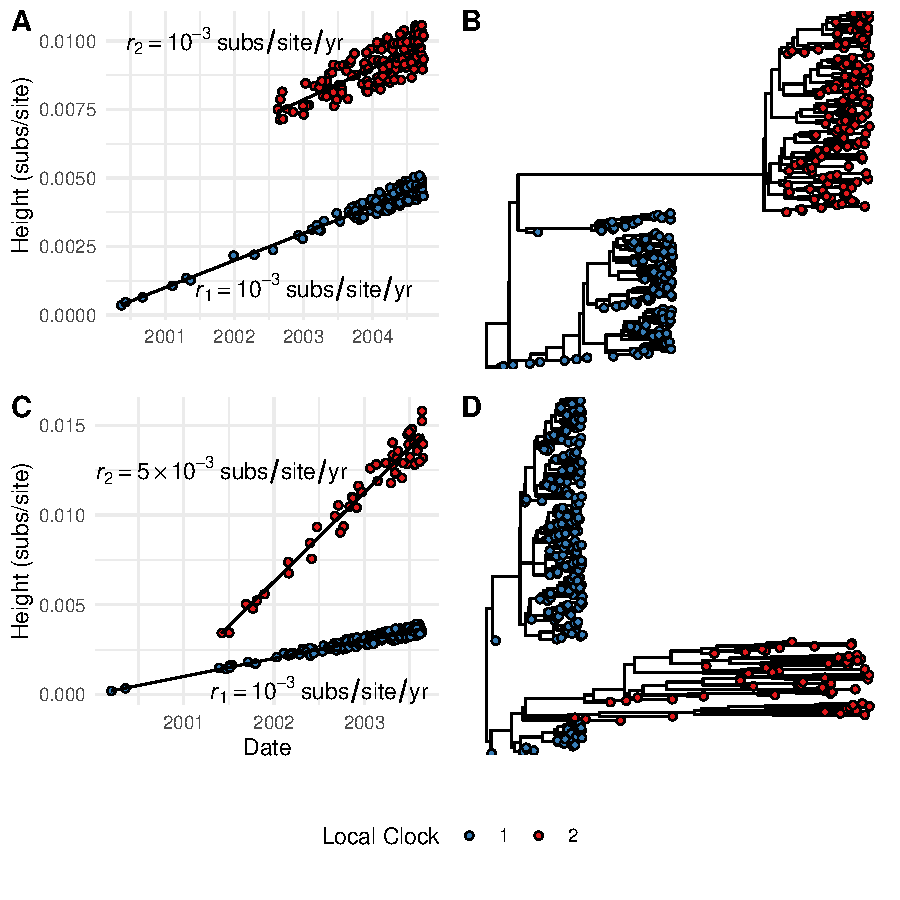
\includegraphics[1\linewidth]{figures/egRTT}
\caption{Simulated examples of how local clocks may manifest in trees and RTT data. (\textbf{A}) RTT data for two local clocks with similar rates separated by a long branch. (\textbf{B})
A tree characteristic of two similar local clock rates separated by a long branch. (\textbf{C}) RTT data where two local clocks have differing evolutionary rates. (\textbf{D}) A tree characteristic of two local clocks with differing rates.}
\label{fig:egRTT}
\end{figure}

\subsection*{General model for global and local strict clocks}
Root to tip regression models strict evolutionary rates as the slope of a linear regression between tip heights and their sampling dates. If we denote the evolutionary rate as $r$ (usually in units of $subs/site/time$), tip heights as $h$ (usually in units of $subs/site$), $o$ as the intercept (interpreted as origin), and sampling times as $t$, then the model for a global strict clock is then of the form:
\begin{equation*}
    h = rt + o + \epsilon
\end{equation*}
where epsilon is the error term.

Clockor2 uses a generalisation of this model to accommodate local clocks. For a given tree with a set of tips $T$, we define local clocks as pertaining to \textit{groups} of tips $g_i$ and a rate parameter for each ($r_i$). For a strict clock model with two local clocks, we then write:
\begin{equation*}
    h = 
    \begin{cases}$
    $r_{1}t + o + \epsilon, \textnormal{ if tip }\in g_1$\\
    $r_{2}t + o + \epsilon, \textnormal{ if tip }\in g_2$
    $
    \end{cases}
\end{equation*}

We refer to \emph{groups} instead of \emph{clades} because while  collections of tips belonging to one local clock are necessarily monophyletic, they do not necessarily comprise a clade. This occurs when two or more local clocks are nested. The tips comprising the outer clock(s) cannot comprise a whole clade if another local clock is nested within it. For example, local clock 1 in Fig. \ref{fig:egRTT} A-B and C-D is not monphyletic because local clock 2 is nested within it.

This general model then captures two key scenarios where local clocks may be appropriate. The first is where rates are similar between local clocks, but separated by a long branch (Fig. \ref{fig:egRTT}A-B). For example, this occurs in the evolution of VOCs in SARS-CoV-2 or due to sparse sampling in the case of ancient \textit{Yersisnia pestis} samples \citet{tay2022emergence, eaton2023plagued}.The second scenario is where rates differ between local clocks \ref{fig:egRTT}C-D). For example, this can occur when a pathogen spreads in different host species, such as has been observed for SARS-CoV-2 in Mink and human hosts \citep{porter2023evolutionary}.

For each group of tips comprising a local clock, we independently conduct an RTT to estimate the slope. $R^2$ values for each clock are then an indication of clock-like behaviour for each local clock. Local clock and global clock configurations can then be compared using an information criterion that combines the likelihood of each local clock's RTT while penalising the number of inferred parameters (3 for each clock - slope, intercept, and variance). Clockor2 allows users to use use either the Bayesian Information Cirterion (BIC), Aikake Information Criterion (AIC), or corrected Aikake Information cirterion (AICc). We reccommend using the BIC because it most heavily penalises the addition of extra parameters, and local clocks in turn.

See supplementary material for derivations of the above information criteria for the local clock model. Briefly, these exploit the assumption independent samples in regression to factor the likelihood across local clocks. Note however that the assumption of independent sampling is flawed because samples necessarily share some ancestry by the assumption of a phylogenetic tree. In other words, ancestral branches are counted over many times in the calculating the height from root to tip for each sample. 


\subsection*{Algorithm for local clock search}
Where it is hypothesised that a datasset contains local clocks, clockor2 provides functionality to corroborate the this hypothesis by performing a search for local clocks in the tree. Briefly, the algorithm takes a maximum number of clocks and a minimum group size for each local clock as input parameters. It then iterates through all combinations of internal nodes from which local clocks can descend to induce local clock configurations satisfying these parameters. Importantly, the clock search algorithm tests for a number of clocks up to an including the maximum number so that more parsimonious configurations with fewer clocks may be found. Configurations are compared using the information criteria outlined above. Again, we recommend the BIC as it penalises additional parameters (ie. additional local clocks) most heavily. See \href{https://github.com/LeoFeatherstone/clockor2Paper/blob/main/figures/clockSearchEg2Clocks.gif}{here for an animation} of the clock search algorithm. 

We stress that this algorithm is intended to corroborate hypotheses about a particular local clock configuration, but is not at all intended to be performed as a blind search. This is because it is highly prone to over-fitting, as outlined later in the results section.

The clock-search algorithm operates in polynomial time (see supplementary material). Efficiency is improved by maximum number of local clocks in the search, increasing the minimum group size, and contingent on the topology of the underlying tree. However, the former two parameters exert a far greater effect on efficiency than topology.

\subsubsection*{clock-search algorithm simulation study}
We conducted a simulation study to test the accuracy of the clock-search algorithm. We started with a core set of 100 simulated trees of 250 tips and added a local clock to a randomly selected node such that it would contain between 50 and 150 tips. For each, we simulated a 5-fold rate increase occurring in either the branch leading to the group/clade, or throughout the group reflecting the two scenarios characterised in Fig \ref{fig:egRTT}. For each of the resulting 200 trees, we applied the clock search algorithm with a minimum group size of 50 tips and a maximum of 2-5 clock. The case of a maximum of 2 clocks tests for baseline accuracy where search parameters match reality. Searches involving a maximum of 3-5 clocks test for over-sensitivity in the algorithm where the maximum number of clocks is inflated. All clock-ssearch tests use the BIC.


\subsection*{Finding the Best Fitting Root}
Clockor2 selects the best fitting root based on the $R^2$ of a global clock model for the input tree. It follows the same algorithm as implemented in Tempest \citet{rambaut_exploring_2016}, but makes use of parallelisation to improve speed for larger trees. Briefly, the tree is rooted along the branch leading to each internal node or tip, an RTT regression is performed, and the root leading to the highest $R^2$ value is selected. When rooting along a branch, clockor2 starts at the midpoint and then optimises the root position using the golden-search-section algorithm.

The best fiting root is inferred using a single, global clock because this presents the most parsimonious model of the evolutionary rate for a given tree. The fit of more elaborate local clock models can then be compared to this using information criteria and/or comparing the $R^2$ values of each model. Clockor2 does not find the best fitting rootf for local clock models.

\subsection*{Dependencies}
Clockor2 has three key dependencies for handling, and plotting trees and RTT data. Trees are handled and manipulated using the phylotree.js library \citep{shank_phylotreejs_2018}. Phylocanvas is used to viaualise trees and plotly.js is used to plot RTT data \citep{abudahab_phylocanvasgl_2021}.



\section*{Results}
\subsection*{Efficiency}
Clockor2 can process trees of up to $10^5$ tips. Finding the best fitting root and the clock-search algorithms make use of parallelisation to increase speed relative to similar RTT tools. Speedup is proportional to the number of threads or cores available. For example, on a 2021 mackbook pro with 16Gb of ram, it took... \textcolor{red}{INSERT STATS ON SPEED OF BFR & CLOCK-SEARCH ONCE BUGS ARE IRONED OUT. MAYBE INCLUDE TABLE OF COMPARISONS TIMES OT TEMPEST}

\subsection*{clock-search accuracy}
\begin{figure}[H]
\centering
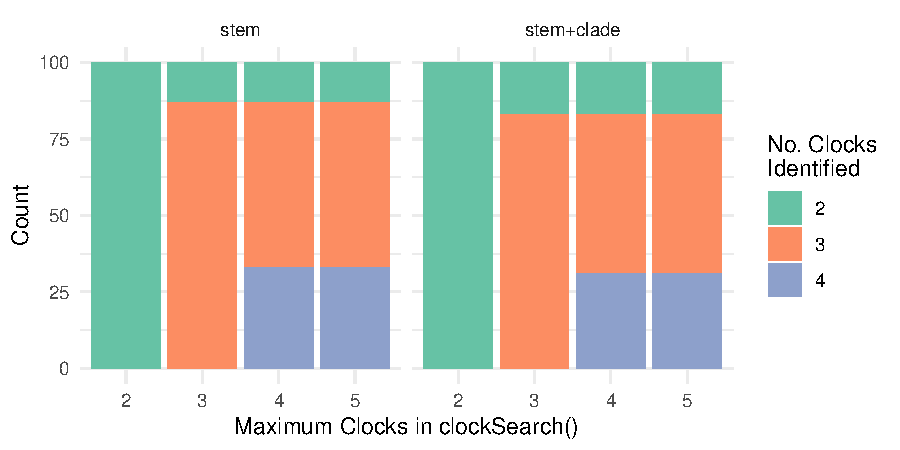
\includegraphics[\linewidth]{figures/inferredClocks.pdf}
\caption{Counts of the number of inferred clocks against the maximum number of clocks allowed by each search. "stem" and "stem+clade" refer to either a rate increase along only the stem of a clade, or with the rate increase continuing in the clade. The true value is 2 and accuracy decreases as the maximum number of clocks allowed by the clock-search algorithm increases.}
\label{fig:simStudy}
\end{figure}

For clock searches with a maximum number of 2 clocks, the clock-search algorithm correctly identified 2 local clocks in the simulated data with complete accuracy (Fig. \ref{fig:simStudy}). However, when the algorithm was allowed to clear for configurations with 3-5 clocks, only 13 and 17 analyses correctly recovered 2 clocks for the stem only and stem+clade rate increases respectively. although the BIC, the most conservative information metric used in clockor2, was used, the clock-search algorithm is still highly prone to over-fitting local clock configurations to data where a higher number of clocks allows for tighter clusters of points in the RTT data can be found.

To this end, we again emphasise that the clock-search algorithm is only intended to be used as a tool testing a number of clocks up to and including the hypothesised number, but never more. It should never be used to blindly search for local clocks with an arbitrarily high number of clocks. For example, to demonstrate intended use we used the clock search with a minimum group size of X and max number of clocks of 2 to test for the presence of two local clocks in SARS-CoV-2 data taken from human and mink hosts in \citet{porter2023evolutionary}. We found that the clock search supported the presence of two clocks dividing mink samples from the Netherlands and the rest of the data, supporting the inference of a second clock for mink hosts. Conversely, improper use would be searching for a number of clocks above the biologically-informed hypothesis of 2.

\section*{Discussion}
- Clockor2 is a flexible framework that is part of the borader shift to web based applications with functionality that can eventually be converted to faster code, such as though bio-rust.
- Future Direction - a pairwise regression that eliminates pseudoreplication in RTT.
- Easier o extend than tempest

\bibliography{clockor2}

\section*{Supplementary Material}
- To Add:
- Derivations for AIC, AICc, and BIC for general strict clock models
- Proof of polynomial time for clockSearch() algorithm.

\end{document}